\documentclass[12pt,a4paper]{article}
\usepackage[utf8]{inputenc}
\usepackage[english,russian]{babel}
\usepackage{indentfirst}
\usepackage{misccorr}
\usepackage{graphicx}
\usepackage{amssymb}
\usepackage{amsmath}

\begin{document}

\begin{center}
    \large
    Теория
    
    Сибгатуллин Булат, Б01-007
    
    \vspace{0.5cm}
    \textbf{Практика применения построения графиков и методов определения параметров теоретической зависимости (данные были взяты из работы 1.3.2).}

\end{center}

\textbf{Формулы используемые при выполнении работы:}

\begin{equation}\label{6}
    M = \frac{\pi R^4 G}{2l}\varphi = f\varphi
\end{equation}

\begin{equation}\label{7}
    f = \frac{\pi R^4 G}{2l}
\end{equation}

\textbf{1.} Познакомимся с установкой, проверим, видно ли в зрительной трубе отражение шкалы в зеркальце. Измерим расстояние($l$) от зеркальца до шкалы, определим диаметр стержня($D$) и шкива($D_{\text{шк}}$).

\vspace{0,5cm}

\begin{tabular}{|c|c|c|c|c|c|c|c|c|c|c|}
\hline
$l$, см & 133,2 & 133,2 & 133,3 & 133,5 & 133,4 & 133,4 & 133,2 & 133,2 & 133,3 & 133,5 \\
\hline
$D$, мм & 5,95 & 5,93 & 5,95 & 5,95 & 5,94 & 5,95 & 5,94 & 5,95 & 5,95 & 5,94 \\
\hline
$R_{\text{шк}}$, см & 10,1 & 10,11 & 10,1 & 10,11 & 10,11 & 10,1 & 10,1 & 10,1 & 10,1 & 10,1 \\
\hline
\end{tabular}

\vspace{0,5cm}

Вычислим средние значения по формуле:

\begin{equation}\label{13}
l = \frac{1}{N} \sum\limits_{\textit{i} = 1}^N l_{\textit{i}}
\end{equation}

Здесь N - это количество измерений, тогда средние значения будут равны:

\[L = 133,32 \: \textit{см} \quad R = 2,973 \: \textit{мм} \quad R_{\text{шк}} = 10,103 \: \textit{см}\]

Систематические погрешности узнаем из характеристик приборо, а случайные вычислим по формуле:

\begin{equation}\label{14}
\sigma_l = \sqrt{\frac{1}{N} \sum\limits_{\textit{i} = 1}^N (l_{\textit{i}} - l)^2}
\end{equation}

\[\sigma_{l_{\text{сист}}} = 0,1 \: \textit{см} \quad \sigma_{l_{\text{сл}}} = 0,37\: \textit{см}\]

\[\sigma_{D_{\text{сист}}} = \sigma_{R_{\text{сист}}} =  0,01\: \textit{мм} \quad \sigma_{D_{\text{сл}}} = \sigma_{R_{\text{сл}}} = 0,002 \: \textit{мм} \]

\[\sigma_{R_{\text{шк сист}}} =  0,05\: \textit{мм} \quad \sigma_{R_{\text{шк сл}}} = 0,02 \: \textit{мм} \]

Зная случайные и систематические погрешности вычислим погрешности измерений по формуле:

\begin{equation}\label{15}
\sigma_l = \sqrt{\sigma_{l_{\text{сист}}}^2 + \sigma_{l_{\text{сл}}}^2}
\end{equation}

\[\sigma_l = 0,38 \: \textit{см} \quad \sigma_{R_{\text{шк}}} = 0,054\:\textit{мм} \quad \sigma_R = 0,01 \: \textit{мм}\]

Увеличивая нагрузку на нитях снимем зависимость \textit{x} = \textit{x(m)}, где \textit{x}, смещение координат на шкале, отражающейся в зеркале, a \textit{m} масса груза, подвешенного на нити:

\vspace{0,5cm}

\begin{tabular}{|c|c|c|c|c|c|c|c|}
\hline
$m$, г & 198 & 396 & 594 & 792 & 594 & 396 & 198 \\
\hline
$x$, см & 9,4 & 17,8 & 26,5 & 34,8 & 27,9 & 17,8 & 9,1 \\
\hline
$x$, см & 9,1 & 17,8 & 26 & 36 & 28 & 17,7 & 9,4 \\
\hline
$x$, см & 9,1 & 17 & 26 & 35 & 27,2 & 17,2 & 9,2 \\
\hline
$x$, см & 9,2 & 17,6 & 25,7 & 34,9 & 28,3 & 17,9 & 9 \\
\hline
\end{tabular}  

\vspace{0,5cm}

Зная \textit{x} и \textit{l} можем посчитать угол $\varphi$ по формуле:

\[ \tan \varphi = \frac{x}{l}\]

По полученным данным построим зависимоть $\varphi = \varphi(\textit{M})$, где $ \textit{M} = \textit{mg}\textit{R}_{\text{шк}}$:

\vspace{0,5cm}

\begin{tabular}{|c|c|c|c|c|c|c|c|}
\hline
$M$, $\text{Н} \cdot \text{м}$ & 0,1962 & 0,3925 & 0,5887 & 0,7850 & 0,5887 & 0,3925 & 0,1962 \\
\hline
$\varphi_1$, рад& 0,0704 & 0,1327 & 0,1962 & 0,2553 & 0,2062 & 0,1327 & 0,0681 \\
\hline
$\varphi_1$, рад& 0,0681 & 0,1327 & 0,1926 & 0,2637 & 0,2070 & 0,1320 & 0,0704 \\
\hline
$\varphi_1$, рад& 0,0681 & 0,1268 & 0,1926 & 0,2567 & 0,2013 & 0,1283 & 0,0689 \\
\hline
$\varphi_1$, рад& 0,0689 & 0,1312 & 0,1904 & 0,2560 & 0,2092 & 0,1335 & 0,0674 \\
\hline
\end{tabular}

\vspace{0,5cm}

Вычислим средние значения $\varphi_1$ по формуле (\ref{13}), для каждого момента сил, и построим таблицу:

\vspace{0,5cm}

\begin{tabular}{|c|c|c|c|c|c|c|c|}
\hline
$M$, $\text{Н} \cdot \text{м}$ & 0,1962 & 0,3925 & 0,5887 & 0,7850 & 0,5887 & 0,3925 & 0,1962 \\
\hline
$\varphi_1$, рад& 0,0688 & 0,1309 & 0,1930 & 0,2579 & 0,2059 & 0,1316 & 0,0687 \\
\hline
\end{tabular}

\vspace{0,5cm}

Угол $\varphi$ используемый в формуле (\ref{6}) равен:

\[\varphi = \frac{\varphi_1}{2}\]

Тогда построим аналогичную таблицу для угла $\varphi$:

\vspace{0,5cm}

\begin{tabular}{|c|c|c|c|c|c|c|c|}
\hline
$M$, $\text{Н} \cdot \text{м}$ & 0,1962 & 0,3925 & 0,5887 & 0,7850 & 0,5887 & 0,3925 & 0,1962 \\
\hline
$\varphi$, рад& 0,0344 & 0,0655 & 0,0965 & 0,1290 & 0,1030 & 0,659 & 0,0344 \\
\hline
\end{tabular}

\vspace{0,5cm}

Погрешность момента сил определяется только погрешностью измерения $R_{\text{шк}}$ и равна:

\[\sigma_M = M_\text{ср}\cdot \frac{\sigma_{R_{\text{шк}}}}{R_{\text{шк}}} = 0,0017 \:\text{Н} \cdot \text{м}\]

Погрешность измерения $\varphi$ будет складываться из случаной и систематической погрешности. Случайную погрешность можем определить по формуле (\ref{14}), а систематическую погрешность по формуле:

\[\frac{\sigma_{\varphi_{\textit{сист}}}}{\varphi} = \sqrt{\Big( \frac{\sigma_x}{x}
\Big) ^2 + \Big( \frac{\sigma_l}{l} \Big) ^2}\]

\vspace{0,5cm}

\begin{tabular}{|c|c|c|c|c|c|c|c|}
\hline
$M$, $\text{Н} \cdot \text{м}$ & 0,1962 & 0,3925 & 0,5887 & 0,7850 & 0,5887 & 0,3925 & 0,1962 \\
\hline
$\sigma_{\varphi_{\textit{сист}}} $, рад& 4,2$\cdot 10^{-4}$ & 5,3$\cdot 10^{-4}$ & 6,6$\cdot 10^{-4}$ & 8,2$\cdot 10^{-4}$ & 6,9$\cdot 10^{-4}$ & 5,3$\cdot 10^{-4}$ & 4,2$\cdot 10^{-4}$ \\
\hline
$\sigma_{\varphi_{\textit{сл}}} $, рад& 9,4$\cdot 10^{-4}$ & 24,2$\cdot 10^{-4}$ & 20,8$\cdot 10^{-4}$ & 33,7$\cdot 10^{-4}$ & 28,9$\cdot 10^{-4}$ & 19,9$\cdot 10^{-4}$ & 11,2$\cdot 10^{-4}$ \\
\hline
\end{tabular}

\vspace{0,5cm}

Погрешность $\sigma_{\varphi}$ найдем по формуле:

\[\sigma_{\varphi} = \sqrt{\sigma_{\varphi_{\text{сл наиб}}} + \sigma_{\varphi_{\text{сист наиб}}}} = 0,0035 \:\text{рад}\]

При помощи метода наименьших квадратов построим график зависимости $\varphi = \varphi(\textit{M})$:

\[\varphi = k\textit{M}\],

Где $k$ найдем по формуле:

\[k = \frac{\langle M \varphi \rangle}{\langle M^2 \rangle} = \frac{0,081}{0,242} = 0,161 \]

По формуле (\ref{6}) определим значение $\textit{f}$:

\[\textit{f} = \frac{1}{k} = 6,253 \: \text{Н} \cdot \text{м}\]

Погрешность $\textit{f}$ будет находиться по формуле:

\[\sigma_{\textit{f}} = \textit{f}\sqrt{\Big(\frac{\sigma_{\varphi}}{\varphi_{\text{ср}}}\Big)^2 + \Big(\frac{\sigma_{M}}{M}\Big)^2} = 0,015 \: \text{Н} \cdot \text{м}\]

Используя формулу (\ref{7}) вычислим значение модуля сдвига \textit{G}:

\[\textit{G} = \frac{6,253 \cdot 2 \cdot 1,3332}{(2,973 \cdot 10^{-3})^4 \cdot 1,1415} = 6,791 \cdot 10^{10} \: \text{Н}/\text{м}^2\]

И погрешность модуля сдвига рассчитаем по формуле:

\[\sigma_{\textit{G}} = \textit{G}\sqrt{\Big(\frac{\sigma_{\textit{f}}}{\textit{f}}\Big)^2 + \Big(\frac{\sigma_{\textit{l}}}{\textit{l}}\Big)^2 + \Big(4\frac{\sigma_{\textit{R}}}{\textit{R}}\Big)^2} = 2,87 \cdot 10^8 \: \text{Н}/\text{м}^2\]

\begin{figure}[h!]
\centering
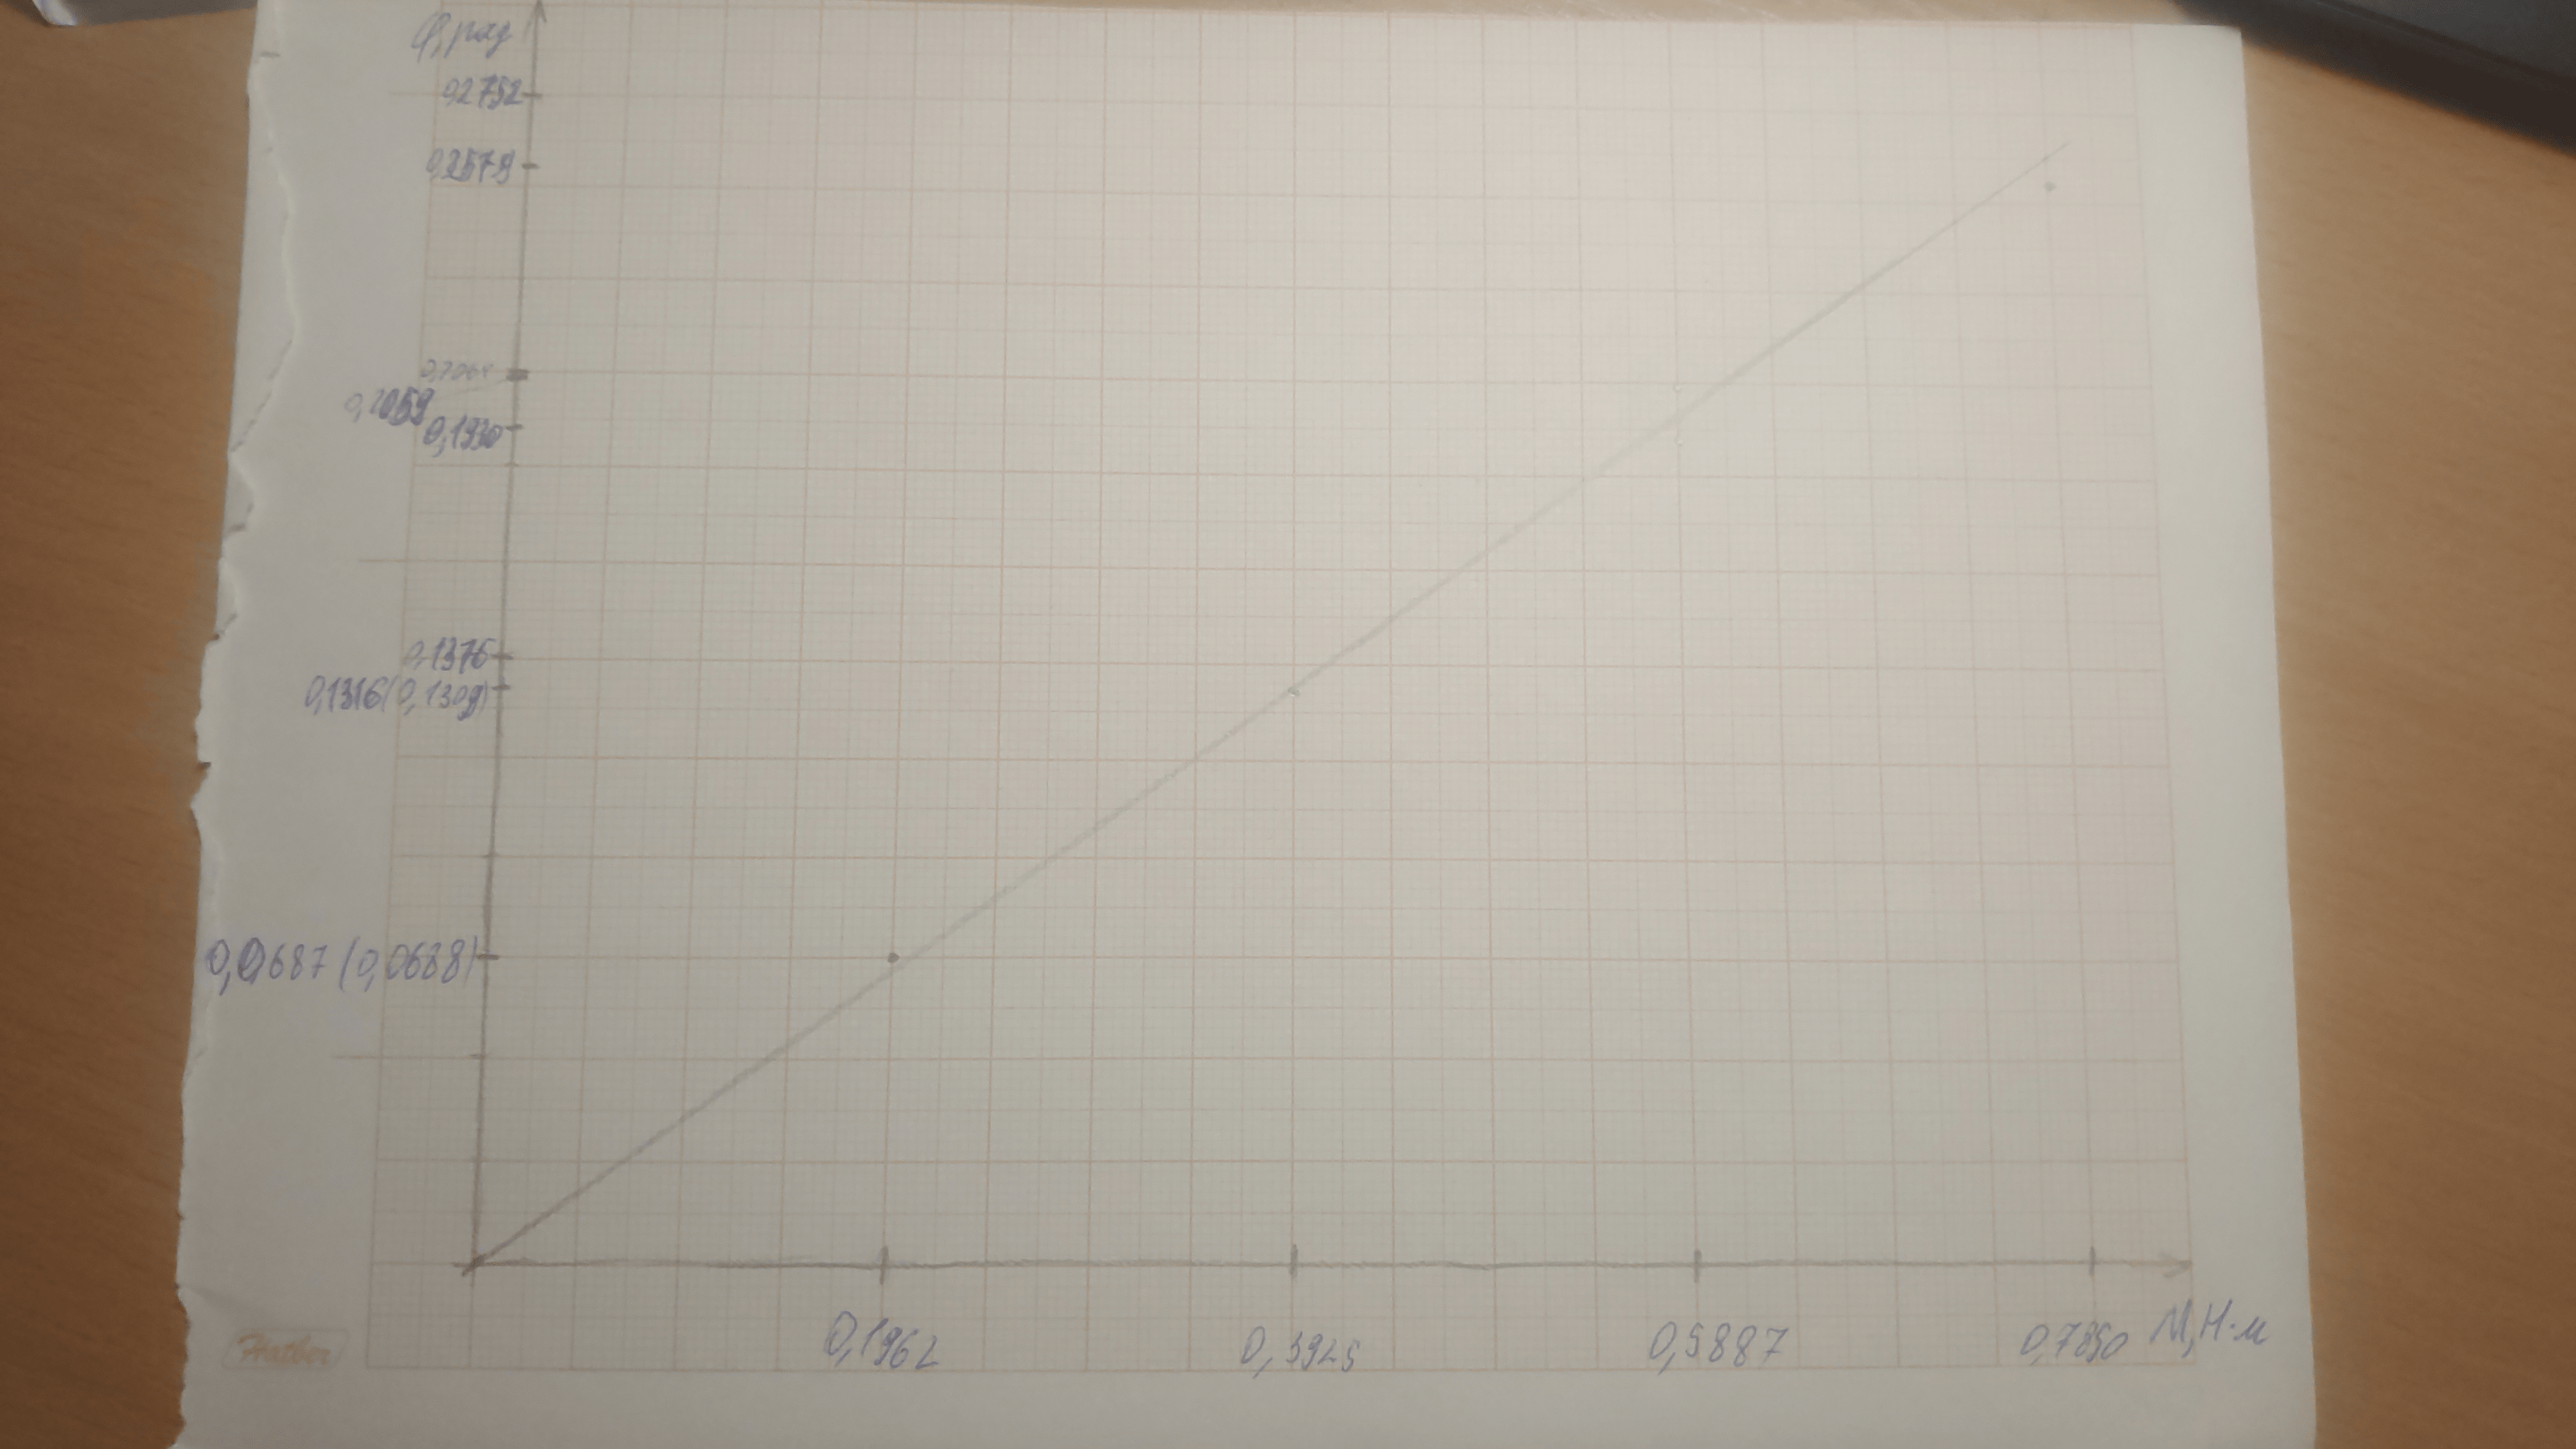
\includegraphics[scale=0.1]{Image2.png}
\caption{График зависимости $\varphi = \varphi(\textit{M})$}
\label{fig:Image1}
\end{figure}

\end{document}